\section{recurrent-event}
\label{sec:recurrent-event}
%%%%%%%%%%%%%%%%%%%%%%%%%%%%%%%%%%%%%%%%%%%%%%%%%%%%%%%%
\begin{figure}[h!]
\begin{center}
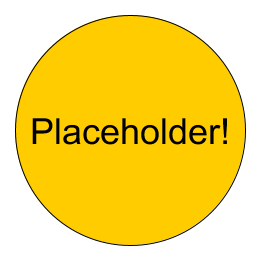
\includegraphics[width=.8\textwidth]{figures/placeholder}
\end{center}
\caption{Schema Diagram for the recurrent-event Pattern. The visual notation is explained in Chapter \ref{chap:prelims}.}
\label{fig:recurrent-event}
\end{figure}
\subsection{Summary}
\label{sum:recurrent-event}
%%%%%%%%%%%%%%%%%%%%%%%%%%%%
A recurrent event series is modelled as an intersection of a collection and a situation. Indeed, a recurrent event is seen as a collection, since it contains entities that share one or more common properties and are unified conceptually (unifying factors). These entities are member of the collection, and are all consecutive events. At the same time, a recurrent event is a situation, intended as a relational context in which the contextualised things are based on a frame: a recurrent event is similar to a plan that defines how the things involved in that plan (i.e. the specific events) shall be carried out, e.g. where the events shall be located, in which time of the year, etc.

%%%%%%%%%%%%%%%%%%%%%%%%%%%%%%%%%%%%%%%%%%%%%%%%%%%%%%%%
\subsection{Axiomatization}
\label{axs:recurrent-event}
%%%%%%%%%%%%%%%%%%%%%%%%%%%%
\begin{align}
% General Axioms\top &\sqsubseteq \forall\textsf{place.Holder} \\ 
\exists\textsf{place.Holder} &\sqsubseteq \top 
% Domain and Range Restrictions\top &\sqsubseteq \forall\textsf{place.Holder} \\ 
\exists\textsf{place.Holder} &\sqsubseteq \top 
% Inverse Aliases (if any)placeholder &\equiv holderplace^- 
\end{align}

%%%%%%%%%%%%%%%%%%%%%%%%%%%%%%%%%%%%%%%%%%%%%%%%%%%%%%%%
\subsection{Explanations}
\label{exp:recurrent-event}
%%%%%%%%%%%%%%%%%%%%%%%%%%%%
\begin{enumerate}
\item temporary item
\end{enumerate}

%%%%%%%%%%%%%%%%%%%%%%%%%%%%%%%%%%%%%%%%%%%%%%%%%%%%%%%%
\subsection{Competency Questions}
\label{cqs:recurrent-event}
%%%%%%%%%%%%%%%%%%%%%%%%%%%%
\begin{enumerate}[CQ1.]
    \item What are the events of a recurrent event series?
    \item Which is the time period elapsing between two events of a recurrent event series?
    \item When is the next event of a recurrent event series scheduled?
    \item What are the unifying criteria shared by all the events in a recurrent event series?
    \item Which is the (immediate) next event in a recurrent event series?
    \item Which is the (immediate) previous event in a recurrent event series?
    \item What is the context or situation of something? 
    \item What are the things present in this context or situation?
\end{enumerate}

\newpage
%%%%%%%%%%%%%%%%%%%%%%%%%%%%%%%%%%%%%%%%%%%%%%%%%%%%%%%%
% End Section
%%%%%%%%%%%%%%%%%%%%%%%%%%%%%%%%%%%%%%%%%%%%%%%%%%%%%%%%
%%%%%%%%%%%%%%%%%%%%%%%%%%%%%%%%%%%%%%%%%%%%%%%%%%%%%%%%